\chapter[Classi]{Classi dei contenuti}

Tutti i contenuti presenti all'interno del sito sono degli oggetti istanze di classi generali che descrivono la forma possibile dei contenuti inseribili. Ad esempio un oggetto di tipo \textsl{folder} è un'istanza della classe \textbf{folder} la quale descrive le proprietà di tutti gli oggetti che da essa derivano. Analiziamo di seguito le classi di contenuto disponibili all'interno del sito e il loro utilizzo.

\section{Classe::Articolo}
La classe Articolo consiste dei seguenti campi:
\begin{description}
\item[Titolo] Il titolo esteso dell'articolo
\item[Titolo Breve] Il titolo breve dell'articolo, se è impostato il nome breve questo ha la precedenza
\item[Autore] Il nome dell'autore dell'articolo, questo parametro è indipendente dal nome di colui che ha effettivamente creato l'oggetto
\item[Introduzione]Una breve introduzione da mostrare nelle viste compatta dell'articolo
\item[Corpo] Il corpo del testo
\item[Abilita commenti] Checkbox per abilitare o meno i commenti
\item[Immagine] Immagine principale dell'articolo
\item[Didascalia immagine] Descrizione del contenuto dell'immagine principale
\item[Data di pubblicazione] Data in cui pubblicare l'articolo, se non viene impostata l'articolo verrà pubblicato istantaneamente
\item[Data di de pubblicazzione] Data in cui rimuovere l'articolo
\item[Parole chiave] Parole chiave (tags) associate all'articolo
\end{description}
Gli oggetti di questa classe possono essere utilizzati per brevi articoli annunci, messaggi etc

\section{Classe::Articolo (pagina principale)}
La classe articolo (pagina principale) consiste dei seguenti campi:
\begin{description}
\item[Titolo] Il titolo esteso dell'articolo
\item[Titolo Breve] Il titolo breve dell'articolo, se è impostato il nome breve questo ha la precedenza
\item[Titolo indice] Il titolo di della prima pagina dell'articolo che comparirà nell'indice
\item[Stile indice] Lo stile dell'indice, per ora sono disponibili tre stili
\item[Autore]L'Autore dell'articolo
\item[Introduzione] Una breve introduzione da mostrare nelle viste ridotte dell'oggetto
\item[Corpo del testo] Testo principale della prima pagina dell'articolo
\item[Immagine] Immagine principale dell'articolo
\item[Didascalia immagine] Descrizione del contenuto dell'immagine principale
\item[Data di pubblicazione] Data in cui pubblicare l'articolo, se non viene impostata l'articolo verrà pubblicato istantaneamente
\item[Data di de pubblicazzione] Data in cui rimuovere l'articolo
\item[Tag] Parole chiave (tags) associate all'articolo
\end{description}
Gli articoli multipagina sono ideali per creare documenti complessi  pof, regolamenti etc. Gli articoli multipagina compaiono nel menu di sinistra e nel menu a tendina fino al terzo livello

\section {Classe::Articolo (pagina successiva)}
Gli oggetti di questa classe possono (e devono) essere creati unicamente come figli di un oggetto Articolo (pagina principale) in quanto rappresentano le pagine secondarie di questo, dalle 2 alla \ldots
La classe Articolo (pagina successiva) consiste dei seguenti campi:
\begin{description}
\item[Titolo] Il titolo esteso dell'articolo
\item[Titolo indice] Il titolo di della pagina n-esima dell'articolo che comparirà nell'indice
\item[Corpo] Testo principale della prima pagina dell'articolo
\item[Tag] Parole chiave (tags) associate all'articolo
\end{description}

\section{Classe::Attributo sondaggio}
La classe Attributo sondaggio viene utilizzata per istanziare oggetti da collegare ad un sondaggio. Tali oggetti sono in grado di contenere del testo xml. I campi a disposizione sono:
\begin{description}
 \item[Descrizione]Testo, immagini inserite dal creatore del sondaggio
\item[Testo] Campo di testo per la risposta
\end{description}

\section{Classe::Calendario}
Gli oggetti della classe calendario vengono utilizzati per creare dei calendari di eventi, tali oggetti possono contenere unicamente degli oggetti di tipo Evento. La classe calendario consiste dei seguenti campi:
\begin{description}
 \item[Calendario] Il nome del calendario
\item[Titolo Breve] Il titolo breve del calendario da usarsi negli alias degli URL
\item[Vista] Il calendairo può essere visualizzato, per mese, per settimana o come agenda.
\item[Gestione prenotazioni]Indica se il calendario viene utilizzato per gestire degli eventi o la prenotazione di degli eventi
\item[Colore] Il colore da attribuire agli eventi nelle viste
\end{description}
\begin{figure}[H]
 \centering
 \includegraphics[width=0.6\textwidth,bb=0 0 546 242]{./immagini/classi/colore_calendario.png}
 % colore_calendario.png: 546x242 pixel, 72dpi, 19.26x8.54 cm, bb=0 0 546 242
 \caption{Selezione del colore degli eventi}
 \label{fig:cal_col}
\end{figure}

\section{Classe::Calendario multiplo}
La classe calendario multiplo viene utilizzata per aggregare più calendari preesistenti all'interno del sito. Durante la visulizzazione è possibile selezionare quali calendari mostrare. La classe calendario consiste dei seguenti campi:
\begin{description}
 \item[Nome]Il nome del calendario multiplo
\item[Descrizione] Una breve descrizione del calendario
\item[Calendari] Una lista (selezionabile  dagli oggetti del sito) dei calendari da visualizzare
\end{description}
\begin{figure}[H]
 \centering
 \includegraphics[width=\textwidth]{./immagini/classi/multicalendario.png}
 % multicalendario.png: 1205x568 pixel, 72dpi, 42.51x20.04 cm, bb=
 \caption{Calendario multiplo visualizzante contemporaneamente quattro calendari}
 \label{fig:multical}
\end{figure}

\section{Classe::Classe}
la classe Classe reppresenta una classe della scuola e funge da contenitore per i materiali prodotti dagli alunni e dai professori a quella classe associati. Tale classe consiste dei seguenti campi:
\begin{description}
\item[Nome] Il nome della classe
\item[Nome breve] Il nome breve della classe
\item[Indirizzo] L'indirizzo:pni, erica, igea, eli etc.
\item[Sezione]La sezione AA, AB AL etc.
\item[Articolata] Spuntate questo campo se la classe è erticolata
\item[Sommario] Una breve descrizione della classe
\item[Descrizione] Descrizione accurata della classe
\item[Informazioni] Zona a blocchi per la presentazione dei contenuti più importanti.
\end{description}
Ogni classe dovrebbe contenere i seguenti elementi minimali:
\begin{figure}[H]
 \centering
 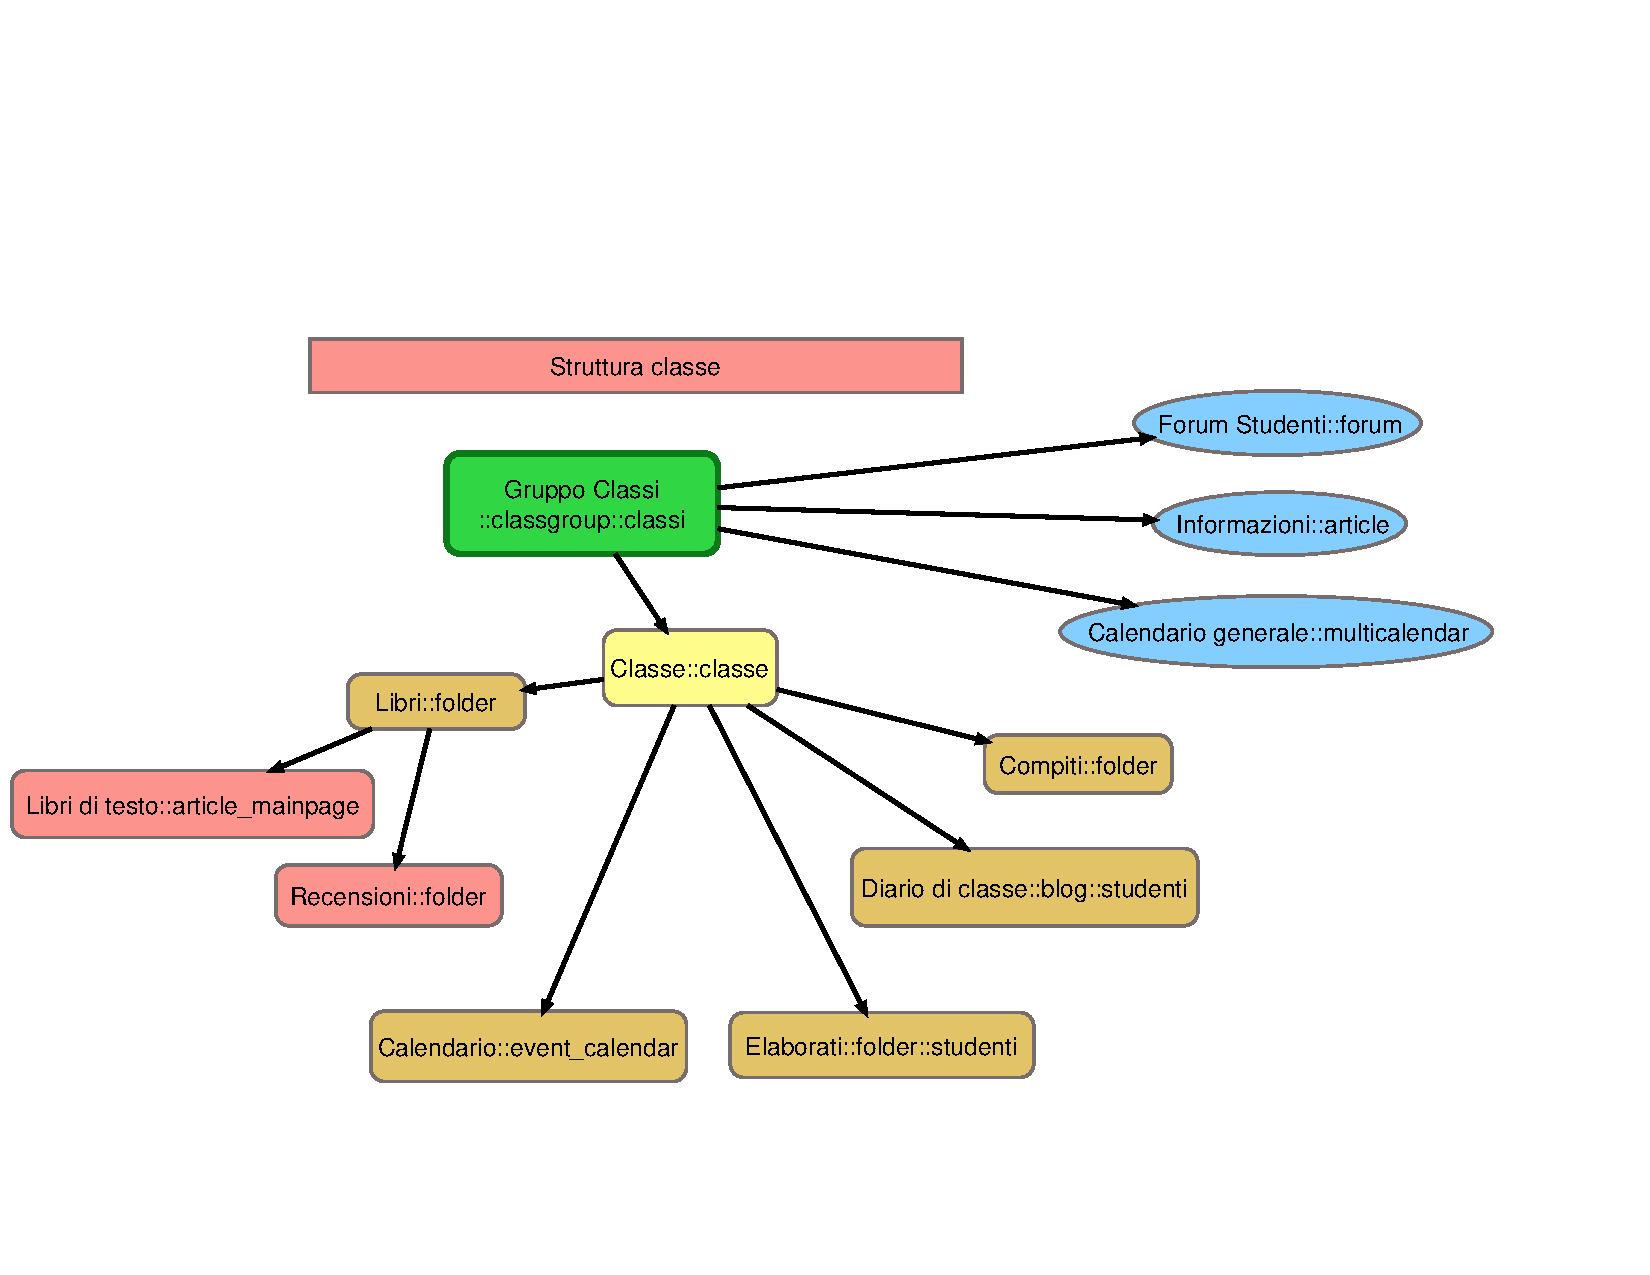
\includegraphics[width=\textwidth]{./immagini/classi/struttura_classe.png}
 % struttura_classe.png: 1455x901 pixel, 72dpi, 51.33x31.79 cm, bb=
 \caption{Struttura base della classe appena dopo la sua creazione}
 \label{fig:strut_class}
\end{figure}

\section{Classe::Commento}
Gli oggetti di questa classe rappresentano dei commenti che gli utenti possono apporre in calce agli articoli. I campi a disposizione sono:
\begin{description}
 \item[Soggetto] Il soggetto del commento
\item[Autore] L'autore del commento
\item[Messaggio]Il messaggio del commento
\end{description}

\section{Classe::Contatti}
La classe contatti deve essere utilizzata per creare delle liste di contatti del personale della scuola. Nomi, indirizzi, numeri di telefono, email etc. Un oggetto di tale classe può aggregare tutti gli oggetti della stessa classe suoi discendenti per ottenere una vista globale dei contatti. La classe Contatti consiste dei seguenti campi:

\begin{description}
 \item[Nome] Il nome esteso della pagina dei contatti
\item[Nome Breve] Il nome breve della pagina dei contatti, attenzione se lo specificate questo ha la precedenza.
\item[Aggrega contatti] Se spuntata questa voce, gli oggeti contatti figli di quello attuale verranno visualizzati nella posizione del genitore.
\item[Note]Informazioni riguardanti la pagina dei contatti
\item[Contatti esterni]Contatti riguardanti soggetti non registrati all'interno del sito
\item[Contatti interni]Contatti riguardanti soggetti registrati all'interno del sito
\end{description}

\section{Classe::Diario}
La classe diario può essere utilizzata come contenitore per brevi articoli. I contenuti in essa inseriti sono ordinati per parola chiave e data di inserimento. All'interno di un contenitore di tipo \textsl{Diario} possono essere inseriti unicamente oggetti della classe dipendente \textsl{Pagina diario}. La classe diario consiste dei seguenti campi:
\begin{description}
 \item[Nome]Il nome del contenitore es. \textsl{Diario Didattico}
\item[Descrizione] Una breve descrizione del contenuto del diario
\item[Parola chiave] Una o più parole chiave per descrivere il diario
\end{description}


\section{Classe::Dipendenti}
La classe dipendenti deve essere utilizzata per creare uno spazio in cui inserire informazioni riguardanti i dipendenti della scuola quindi Insegnanti, Personale Ata, Dsga e presidenza.I campi disponibili per questa classe sono:
\begin{description}
 \item[Nome] Il nome dell'oggetto es. \textsl{Docenti}
\item[Sommario]Un breve sommario circa i contenuti della sezione
\item[Logo]Un logo per rappresentare graficamente il gruppo di dipedenti
\item[Descrizione]Una descrizione più ampia dei contenuti della sezione
\item[Mostra oggetti figli]Visualizza gli elementi figli dell'oggetto Dipendeti
\item[Mostra extra info]Visualizza una barra laterale in cui inserire ulteriori informazioni
\end{description}


\section{Classe::Evento}
Un oggetto di questa classe deve essere obbligatoriamente contenuto da un oggetto calendario. Un oggetto evento rappresenta un entrata all'interno del calendario. È possibile specificare accadimenti sempli o con ripetizione.
I campi di questa classe sono:
\begin{description}
 \item[Titolo breve] Il titolo dell'evento visualizzato all'interno del calendario
\item[Titolo]Il titolo dell'evento mostrato nella vista completa
\item[Testo]Il testo dell'evento
\item[Categoria] La categoria a cui appartiene l'evento (tag)
\item[Da]La data di inizio dell'evento
\item[a]La data di fine dell'evento
\item[Frequenza]La frequenza di ripetizione dell'evento
\item[Fine ripetizione]Quando l'evento smette di ripetersi
\end{description}

\section{Classe::Folder}
La classe Folder deve essere utilizzata come elemento generico per la creazione di gerarchie all'interno del sisto analogamento a quanto viene fatto sul filesystem con una Directory. I campi di questa classe sono:
\begin{description}
 \item[Nome breve] Nome breve da usare nell'url e nelle viste compatte
\item[Nome]Nome del folder
\item[Icona] Icona da visualizzare nelle viste compatte
\item[Sommario]Breve introduzione dei contenuti
\item[Descrizione]Descrizione ampia dei contenuti
\item[Mostra sotto elementi]Mostra gli elementi figli
\item[Mostra extra info]Mostra una barra con ulteriori contenuti
\item[Tags]Parole chiave per descrivere i contenuti
\end{description}


\section{Classe::Folder circolari}
Il folder circolari è un elemento contenitore per le circolari emanate dalla scuola. I file contenuti all'interno di un folder circolari sono consultabile temporalmente, ovvero nella barra di destra è presente un calendario che permette all'utente di visualizzare solo quelle circolari emesse in specifi intervalli temporali.
\begin{figure}[H]
 \centering
 \includegraphics[width=\textwidth]{./immagini/classi/folder_circolari.png}
 % folder_circolari.png: 1089x236 pixel, 72dpi, 38.42x8.33 cm, bb=
 \caption{Organizzazione dei contenuti all'interno di un folder circolari}
 \label{fig:folder_circolari}
\end{figure}

I campi a disposizione di questa classe sono:
\begin{description}
 \item[Nome] Nome completo del folder
\item[Nome breve] Nome breve del folder
\item[Sommario] Sommario da mostrare nelle viste compatte
\item[Descrizione] Descrizione più dettagliata dei contenuti
\item[Logo]Logo da mostrare nelle viste compatte
\item[Tags]Parole chiave
\end{description}

\section{Classe::Folder Documenti}
Gli oggetti della classe Folder Documenti devono essere utilizzati come contenitori di file: moduli, prestampati etc. e mai come contenitori generici. I campi a disposizione di questa classe sono:
\begin{description}
\item[Nome] Il nome completo dell'unità organizzativa
\item[Nome breve]  Il nome compatto dell'unità organizzativa
\item[Icona]Un'icona per le viste compatte dell'oggetto
\item[Sommario] Un breve sommario per descrivere i contenuti del folder
\item[Mostra sotto elementi] Visualizza gli oggetti contenuti, in questo caso file e altri Folder Documenti
\item[Mostra extra info]Mostra informazioni aggiuntive sulla destra
\end{description}

\section{Classe::Formulario Feedback}
Il formulario può essere utilizzato da un utente per creare una pagina per comunicare con i visitatori del sito. Durante la creazione di un oggetto appartenente a questa classe, l'editore deve fornire un suo valido indirizzo e-mail al quale i messaggi dei visitatori saranno.
\begin{figure}[H]
 \centering
 \includegraphics[width=\textwidth]{./immagini/classi/feedback.png}
 % feedback.png: 1234x593 pixel, 72dpi, 43.53x20.92 cm, bb=
 \caption{Il creatore dell'oggetto deve fornire la sua e-mail durante la crazione del formulario per il feedback}
 \label{fig:feedback}
\end{figure}
I campi a disposizione di questa classe sono:
\begin{description}
\item[Nome] Il nome del formulario
\item[Descrizione] Una breve descrizione dello scopo del formulario
\item[Nome*]Campo che dovrà essere compilato dall'utente con il suo nome al momento dell'invio del formulario
\item[Soggetto]Il soggetto del messaggio dell'utente
\item[Messaggio] Il corpo del messaggio che l'utente vuole inviare
\item[E-mail]L'email dell'utente (se vuole essere ricontattato)
\item[E-mail destinatario]L'email di colui che crea l'oggetto. A questo indirizzo verranno inviati i messaggi scritti dagli utenti
\end{description}

\section{Classe::Forum}
La classe Forum deve essere utilizzata per creare un forum, gli oggetti di tale classe possono essere figli di un oggetto raccoglitore di forum di classe Forums. I campi a disposizione sono:
\begin{description}
\item[Nome] Il nome da assegnare al forum
\item[Descrizione] Una breve descrizione dei contenuti del forum
\end{description}

\section{Classe::Forum-argomento}
Gli oggetti di questa classe sono unicamente figli di un oggetto di classe Forum e devono essere utilizzati per creare delle discussioni all'interno  di un forum.
I campi a disposizione sono:
\begin{description}
 \item[Soggetto]L'argomento su cui verte la discussione
\item[Messaggio]Una domanda da rivolgere ai membri del forum
\item[In evidenza]L'argomento viene posto in evidenza all'interno del forum (compare tra i primi elementi)
\item[Notificami] Avvertimi se qualcuno risponde alla mia domanda
\end{description}

\section{Classe::Forum-risposta}
Gli oggetti di questa classe devono essere figli di un oggetto Forum-argomento e sono utilizzati per rispodenre alle domande che altri utenti hanno posto tramite un oggeto Forum-argomento. I campi a disposizione sono:
\begin{description}
 \item[Soggetto]Il soggetto della risposta
\item[Messaggio]Il messaggio della risposta
\end{description}

\section{Classe:Forums}
Gli oggetti di questa classe fungono da contenitori di Forum. I campi a disposizione sono:
\begin{description}
\item[Titolo]Il titolo del contenitore di forum
\item[Descrizione] Una breve descrizione dei contenuti dei forum
\end{description}

\section{Classe::Frontpage}
Gli oggetti di classe Frontpage vengono utilizzati per presentare notizie ed informazioni presenti all'interno del sito. Si rimanda al capitolo frontpage per una descrizione completa circa il loro utilizzo. I campi a disposizione sono:
\begin{description}
 \item[Nome] Il nome completo della frontpage
\item[Struttura]Il campo struttura in cui inserire le informazioni provenienti da altre sezioni del sito
\item[Etichette]Delle etichette con cui descrivere i contenuti
\end{description}

\section{Classe::Frontpage m2000}
Questa classe rappresenta un'evoluzione della classe Frontpage. Oltre al campo struttura per cui rimandiamo al capitolo sulla gestione delle frontpage è possibile inserire una descrizione in testa alla pagina, visualizzare un menu sulla sinistra e gli oggetti figli sul fondo della pagina. I campi a disposizione sono:
\begin{description}
\item[Nome] Il nome della frontpage
\item[Descrizione] Una breve descrizione dei contenuti (opzionale)
\item[Struttura]La struttura in cui inserire informazioni provenienti da altre parti del sito
\item[Etichette]Delle etichette per descrivere i contenuti
\item[Mostra menu]Visualizza o meno il menu sulla sinistra
\item[Mostra sotto elementi]Mostra gli oggetti figli
\item[Logo]Un logo da visualizzare nelle viste ridotte
\item[Piè di pagina]Testo e annotazioni da inserire nel piè di pagina
\end{description}

\section{Classe::Frontpage scuola}
Questo tipo di frontpage deve essere utilizzato per la creazione delle pagine principali di ognuna delle scuole costituenti l'istituto. I campi a disposizione sono:
\begin{description}
\item[Descrizione] Una breve descrizione della scuola che verrà posizionata in testa alla pagina
\item[Titolo]Il nome della scuola
\item[Coordinatore di sede]Il nome del coordinatore di sede
\item[Codice meccanografico]Il codice meccanografico della scuola
\item[Logo]Il logo dalla scuola come apparirà nel menu a blocchi in alto 
\item[Foto scuola]La foto della scuola
\item[Pagina]La struttura della pagina in cui pubblicare i contenuti preseti all'interno della sezione della scuola
\item[Piè di pagina]Del testo e delle note da riportare in piè di pagina
\end{description}

\section{Classe::Galleria}
Gli oggetti di questa classe devono essere utilizzati per creare gallerie di immagine e video in formato flv. I campi a disposizione sono:
\begin{description}
 \item[Nome]Il nome della galleria
\item[Breve descrizione]Una breve descrizione per le viste compatte
\item[Descrizione]Una descrizione completa per la vista totale della galleria
\item[Immagini]Un'immagine da usare come frontespizio della galleria
\item[Icona]Una piccola immagine per la visualizzazione ad icona della galleria
\item[Anno scolastico]L'anno scolastico in cui le immagini sono state fatte
\item[Mostra sotto gallerie] Visualizza le gallerie secondarie
\end{description}

\section{Classe::gruppoClassi}
Gli oggetti di questa classe fungono da aggregatori di Classi (della scuola). Vengono utilizzati per presentare l'insieme di tutte le classi del corrente anno scolastico di ogni scuola. I campi a disposizione sono:
\begin{description}
\item[Nome]Il nome del gruppo di classi
\item[Nome breve]Un nome breve da mostrare nelle viste compatte e nell'url
\item[Sommario]Un breve sommario da mostrare nelle viste compatte
\item[Descrizione]La descrizione delle classi della scuola
\item[Mostra extra info]Se mostrare  o meno una barra a destra con informazioni aggiuntive
\item[Tags]Etichette che descrivono il contenuto
\end{description}

\section{Classe::gruppoDocenti}
Gli oggetti di tale classe vengono utilizzati come raccoglitori degli spazi personali dei docenti. I campi a disposizione sono:
\begin{description}
 \item[Nome]Il nome del gruppo di docenti
\item[Nome breve]Un nome breve da mostrare nelle viste compatte
\item[Sommario]Il sommario da mostrare nelle viste compatte
\item[Descrizione]Un descrizione più completa da mostrare nelle viste totali
\end{description}

\section{Classe::Colonna info}
Gli oggetti di questa classe possono essere utilizzati per fornire in una colonna sulla destra dei contenuti delle informazioni aggiuntive. Si rimanda al capitolo ad esse dedicato per ulteriori informazioni. I campi a disposizione sono:
\begin{description}
 \item[Titolo] Il nome della colonna di informazioni
\item[Immagine] Un'immagine con cui aprire la colonna
\item[Url immagine] Un link da associare all'immagine
\item[Contenuto] Il testo delle informazioni aggiuntive che si vogliono dare
\item[Url] Un link da associare alle informazioni
\end{description}

\section{Classe:Layout Globale}
Gli oggetti di questa classe possono essere utilizzati per fornire in una colonna sulla destra dei contenuti delle informazioni aggiuntive. Si rimanda al capitolo ad esse dedicato per ulteriori informazioni. I campi a disposizione sono:
\begin{description}
 \item[Nome]Il nome della colonna di informazioni
\item[Blocchi] Colonna per pubblicare contenuti correlati
\end{description}

\section{Classe::Libro}
Gli oggetti di questa classe rappresentano dei libri e possono essere utilizzati per, ad esempio, inserire i libri della biblioteca scolastica. I campi a disposizione sono:
\begin{description}
\item[Titolo]Il titolo del libro
\item[Autore]L'autore o gli autori separati da una virgola del libro
\item[Casa editrice]La casa editrice del libro
\item[Copertina]Un'immagine della copertina del libro
\item[Descrizione]Descrizione del libro
\item[Isbn]Il codice isbn del libro
\end{description}

\section{Classe::Link}
Gli oggetti di questa classe vengono utilizzati per creare dei collegamenti a risorse esterne al sito es. il sito del ministero della pubblica istruzione. I campi a disposizione sone:
\begin{description}
 \item[Nome] Il nome del link
\item[Descrizione] Una breve descrizione delle risorse raggiungibili seguendo il link
\item[Indirizzo]L'url del link
\end{description}

\section{Classe::Macroarea}
Gli oggetti di questo tipo fungono da frontpage per le macroare. Un oggetto di tipo Frontpage dovrebbe contenere unicamente oggetti di tipo Frontpage. I campi disponibili sono:
\begin{description}
 \item[Titolo]Il nome della macroarea
\item[Descrizione]Una descrizione dei contenuti della zona
\item[Pagina]Un elemento contenitore di blocchi per il cui utilizzo rinviamo alla sezione frontpage
\item[Logo]Un'immagine da mostrare nella vista ad icone 
\item[Referente]Il referente della macroarea da selezionare tra gli iscritti al sito
\item[Mostra menu]Se mostrare o meno il menu sulla sinistra
\item[Mostra figli]Se mostrare o meno gli oggetti figli
\end{description}

\section{Classe::Pagina diario}
Gli oggetti di questa classe rappresentano dei brevi articoli che andranno a costituire le pagine di un diario. Tali oggetti potranno essere unicamente figli di un padre di classe Diario. Le classi Diario e Pagina diario sono quindi utilizzate per cotruire l'analogo di un \textsl{Blog}. I campi a disposisizione sono:
\begin{description}
 \item[Titolo] Il titolo della pagine di diario
\item[Corpo] Il corpo del testo
\item[Data di pubblicazione] La data in cui il contenuto verrà reso pubblicamente disponibile
\item[Data di de pubblicazione]La data in cui il contenuto non sarà più pubblicamente disponibile
\item[Parole chiave]Le parole chiave da associare al contenuto
\item[Abilita commenti] Campo per abilitare la possibilità di commentare il contenuto.
\end{description}

\section{Classe::Professore (spazio personale)}
Gli oggetti di questa classe vengono creati automaticamente durante il processo di registrazione di un insegnate. Essi rappresentano dei contenitori all'interno dei quali i docenti potranno caricare i propri materiali didattici. Per una descrizione più approfondita rimandiamo al capitolo correlato. I campi a disposizione sono:
\begin{description}
\item[Nome]Il nome del docente (auto assegnato durante la creazione dell'account)
\item[Nome breve]Un nome breve da usare nelle viste compatte
\item[Telefono]Il numero di telefono del docente
\item[Email]L'email del docente (distinta o uguale a quella di registrazione)
\item[Ruolo]Il ruolo del docente: vicepreside, collaboratore etc.
\item[Descrizione]Una descrizione del docente
\item[Mostra sotto elementi]Se mostrare o meno i contenuti figli in calce
\item[Tags]Delle etichette per categorizzare il docente
\end{description}

\section{Classe::Progetto}
Gli oggetti di questa classe devono essere utilizzati per creare un contenitore per i progetti e devono essere preferibilmente inseriti in un Folder. I campi a disposizione sono:
\begin{description}
 \item[Titolo] Il titolo completo del progetto
\item[Titolo breve] Un titolo breve per il progetto da mostrare nelle viste compatte
\item[Docenti responsabili] I docenti responsabili del progetto da selezionare tra i docenti registrati
\item[Codice progetto] Il codice del progetto fornito dalla segreteria
\item[Autore] L'autore del contenuto
\item[Introduzione]Breve introduzione del progetto da mostrare nelle viste compatte
\item[Corpo]Il corpo del testo del progetto
\item[Logo]Il logo del progetto per le viste compatte
\item[Mostra figli]Se mostrare gli oggetti figli dell'oggetto contenitore progetto
\item[Parola chiave]Una o più parole chiave per descrivere i contenuti del progetto
\end{description}

\section{Classe::Questionario (breve)}
Classe per creare dei sondaggi breve (una singola domanda). Tali oggetti possono essere inseriti, ad esempio, nella pagina principale del sito. I campi a disposizione sono:
\begin{description}
\item[Nome]Il nome del sondaggio breve
\item[Descrizione]La descrizione del sondaggio
\item[Domanda]Il testo della domanda
\end{description}

\section{Classe::Raccoglitore circolari}
Gli oggetti di questa classe sono utilizzati come contenitori di oggetti del tipo Folder Circolari. I campi a disposizione sono:
\begin{description}
\item[Nome] Il nome del direttorio per le circolari
\item[Nome Breve]Un nome breve da utilizzare nelle viste compatte
\item[Sommario]Un sommario da mostrare nelle viste compatte
\item[Descrizione]La descrizione per le viste totali
\item[Mostra extra info]Se mostrare o meno una barra sulla destra con ulteriori informazioni
\item[Tags]Delle etichette per categorizzare il contenuto.
\end{description}

\section{Classe::Sondaggio}
Gli oggetti di questa classe sono utilizzati per creare sondaggi complessi. Per una descrizione approfondita del loro utilizzo rimandiamo al capitolo corrispondente. I campi a disposizione sono:
\begin{description}
\item[Nome]Il nome del sondaggio
\item[Logo]Un'immagine da mostrare nelle viste compatte e nella vista totale
\item[Descrizione]Un breve descrizione del sondaggio
\item[Sondaggio]Il sondaggio multi domanda
\end{description}

\section{Classe::Ufficio}
Gli oggetti di questa classe vengono usati per rappresentare gli uffici della scuola. 
\begin{description}
\item[Nome] Il nome dell'ufficio
\item[Responsabile ufficio]Il nome del responsabile dell'ufficio
\item[Logo]Un'immagine per le viste ad icona
\item[Attività ufficio]Il tipo di attività dell'ufficio
\item[Contatti ufficio] I contatti del personale dell'ufficio
\item[In evidenza]Gli elementi in evidenza, campo a blocchi	
\end{description}



